\documentclass[border=5mm]{standalone}
    \usepackage {tikz}
    \usepackage{amssymb}

    \begin{document}
    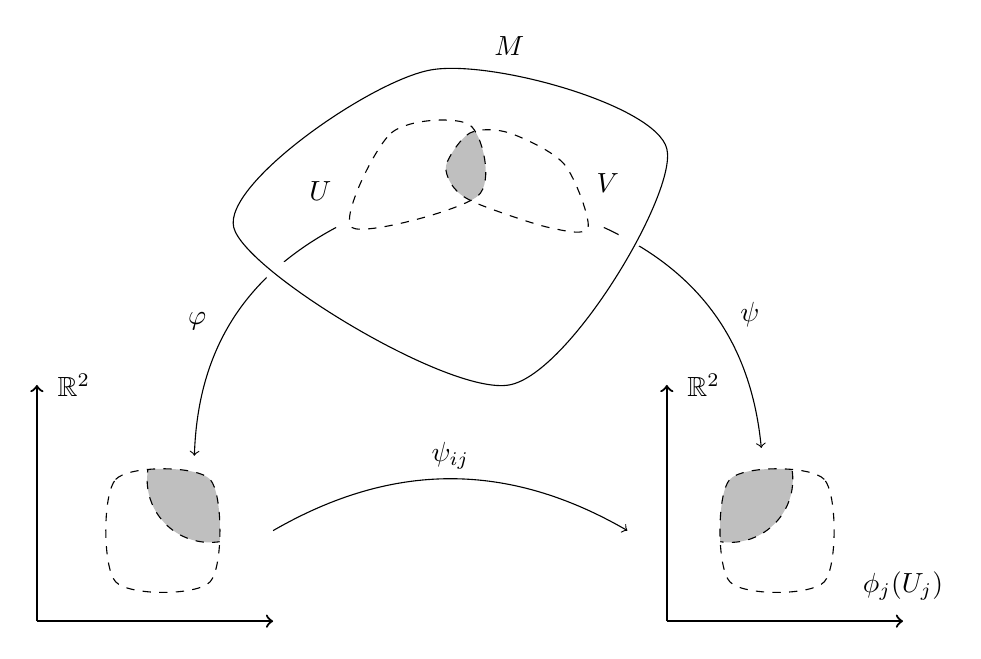
\begin{tikzpicture}

    % Functions i
    \path[->] (0.8, 0) edge [bend right] node[left, xshift=-2mm] {$\varphi$} (-1, -2.9);
    \draw[white,fill=white] (0.06,-0.57) circle (.15cm);

    % Functions j
    \path[->] (4.2, 0) edge [bend left] node[right, xshift=2mm] {$\psi$} (6.2, -2.8);
    \draw[white, fill=white] (4.54,-0.12) circle (.15cm);

    % Manifold
    \draw[smooth cycle] plot coordinates{(2,2) (-0.5,0) (3,-2) (5,1)} node at (3,2.3) {$M$};

    % Subsets
    \begin{scope}
        \clip[smooth cycle] plot coordinates {(1,0) (1.5, 1.2) (2.5,1.3) (2.6, 0.4)};
        \fill[gray!50, smooth cycle] plot coordinates {(4, 0) (3.7, 0.8) (3.0, 1.2) (2.5, 1.2) (2.2, 0.8) (2.3, 0.5) (2.6, 0.3) (3.5, 0.0)};
    \end{scope}
    \draw[dashed, smooth cycle] plot coordinates {(1,0) (1.5, 1.2) (2.5,1.3) (2.6, 0.4)}
    node [label={[label distance=-0.3cm, xshift=-2cm, fill=white]:$U$}] {};
    \draw[dashed, smooth cycle] plot coordinates {(4, 0) (3.7, 0.8) (3.0, 1.2) (2.5, 1.2) (2.2, 0.8) (2.3, 0.5) (2.6, 0.3) (3.5, 0.0)} node [label={[label distance=-0.8cm, xshift=.75cm, yshift=1cm, fill=white]:$V$}] {};

    % First Axis
    \draw[thick, ->] (-3,-5) -- (0, -5)  {};
    \draw[thick, ->] (-3,-5) -- (-3, -2) node [label=right:$\mathbb{R}^2$] {};

    % Arrow from i to j
    \path[->] (0, -3.85) edge [bend left]  node[midway, above]{$\psi_{ij}$} (4.5, -3.85);

    % Second Axis
    \draw[thick, ->] (5, -5) -- (8, -5) node [label=above:$\phi_j(U_j)$] {};
    \draw[thick, ->] (5, -5) -- (5, -2) node [label=right:$\mathbb{R}^2$] {};

% Sets in R^m
\begin{scope}
    \clip [smooth cycle] plot coordinates{(-2, -4.5) (-2, -3.2) (-0.8, -3.2) (-0.8, -4.5)};
    \draw[fill=gray!50, dashed] (-0.8, -3.2) circle (0.8);
\end{scope}
\draw [smooth cycle, dashed] plot coordinates{(-2, -4.5) (-2, -3.2) (-0.8, -3.2) (-0.8, -4.5)};

\begin{scope}
    \clip [smooth cycle] plot coordinates{(7, -4.5) (7, -3.2) (5.8, -3.2) (5.8, -4.5)};
    \draw[fill=gray!50, dashed] (5.8, -3.2) circle (0.8);
\end{scope}
\draw[smooth cycle,dashed] plot coordinates{(7, -4.5) (7, -3.2) (5.8, -3.2) (5.8, -4.5)};
\end{tikzpicture}

\end{document}
